% =====================================================================
% Capítulo: Análisis del Sistema
% Fuentes: borradores/04-analisis.tex, docs/tfg/REQUISITOS.md,
% apps/web/supabase/schemas/*.sql, apps/e2e/tests, DECISIONES.md.
% Estado de las fuentes: F3c cerrada.
% =====================================================================

Este capítulo analiza el comportamiento esperado del sistema a partir de los
requisitos del capítulo anterior. Se presentan el modelo de casos de uso, con
la especificación de los principales, el modelo conceptual de datos y las
reglas de negocio que el sistema debe respetar.

% ---------------------------------------------------------------------
\section{Modelo de casos de uso}
\label{sec:ana-casos-uso}

Se han seleccionado ocho casos de uso principales que recorren todos los
módulos de la plataforma y que sirven de base para su validación
(tabla~\ref{tab:ana-cu} y figura~\ref{fig:ana-casos-uso}). Cada uno tiene una
o varias pruebas E2E que lo ejercitan (capítulo de Pruebas).

\begin{table}[htbp]
  \centering
  \footnotesize
  \caption{Casos de uso principales.}
  \label{tab:ana-cu}
  \begin{tabularx}{\textwidth}{@{}l>{\raggedright\arraybackslash}p{2.6cm}X>{\raggedright\arraybackslash}p{2.4cm}@{}}
    \toprule
    \textbf{CU} & \textbf{Actor principal} & \textbf{Descripción} & \textbf{Requisitos} \\
    \midrule
    CU-01 & Visitante & Se registra, verifica el correo y accede al área privada & RF-01, RF-03 \\
    CU-02 & Usuario & Crea un equipo e invita a un empleado con el rol \textit{member} & RF-06 \\
    CU-03 & Propietario del equipo & Contrata un plan y el estado de la suscripción se refleja en la aplicación & RF-07 \\
    CU-04 & Miembro sin permiso & Intenta gestionar la facturación y se le deniega en la interfaz, en el servidor y en la base de datos & RF-06, RNF-02, RNF-03 \\
    CU-05 & Super-administrador & Busca un usuario, lo bloquea y lo suplanta para darle soporte & RF-08 \\
    CU-06 & Personal del CMS & Edita registros de una tabla según sus permisos; la acción queda auditada & RF-09, RF-10 \\
    CU-07 & Desarrollador & Arranca un producto nuevo a partir de PymeKit cambiando solo la configuración & RNF-01, RNF-07 \\
    CU-08 & Personal del CMS & Publica una entrada del blog desde la consola, que el visitante lee en la web pública & RF-01, RF-09 \\
    \bottomrule
  \end{tabularx}
\end{table}

\begin{figure}[htbp]
  \centering
  \resizebox{\textwidth}{!}{%
  \begin{tikzpicture}[
      font=\footnotesize,
      uc/.style={ellipse, draw, minimum width=4.6cm, minimum height=0.85cm,
                 align=center, inner sep=1pt},
      lbl/.style={align=center, font=\footnotesize\bfseries},
      link/.style={-},
      actor/.pic={
        \draw (0,0.42) circle (0.13);
        \draw (0,0.29) -- (0,-0.05);
        \draw (-0.22,0.17) -- (0.22,0.17);
        \draw (0,-0.05) -- (-0.17,-0.38);
        \draw (0,-0.05) -- (0.17,-0.38);
      }
    ]
    % Casos de uso
    \node[uc] (cu1) at (0, 4.2)  {CU-01 Registrarse y\\acceder al área privada};
    \node[uc] (cu2) at (0, 3.0)  {CU-02 Crear equipo\\e invitar a un miembro};
    \node[uc] (cu3) at (0, 1.8)  {CU-03 Contratar\\un plan};
    \node[uc] (cu4) at (0, 0.6)  {CU-04 Gestionar la\\facturación (denegado)};
    \node[uc] (cu5) at (0, -0.6) {CU-05 Bloquear y\\suplantar a un usuario};
    \node[uc] (cu6) at (0, -1.8) {CU-06 Editar registros\\en el CMS (auditado)};
    \node[uc] (cu8) at (0, -3.0) {CU-08 Publicar una\\entrada del blog};
    \node[uc] (cu7) at (0, -4.2) {CU-07 Arrancar un\\producto nuevo};

    \begin{scope}[on background layer]
      \node[draw, rounded corners, fit=(cu1)(cu7), inner sep=12pt,
            label={[font=\small\bfseries]above:PymeKit}] (sys) {};
    \end{scope}

    % Actores de la izquierda (clientes)
    \pic at (-6.2, 4.0) {actor};  \node[lbl] (vis) at (-6.2, 3.3)  {Visitante};
    \pic at (-6.2, 2.0) {actor};  \node[lbl] (usu) at (-6.2, 1.3)  {Usuario};
    \pic at (-6.2, 0.0) {actor};  \node[lbl] (pro) at (-6.2, -0.75) {Propietario\\del equipo};
    \pic at (-6.2, -2.2) {actor}; \node[lbl] (mie) at (-6.2, -2.95) {Miembro\\sin permiso};

    % Actores de la derecha (personal y sistemas externos)
    \pic at (6.2, 2.4) {actor};   \node[lbl] (pas) at (6.2, 1.7)  {Pasarela\\de pago};
    \pic at (6.2, 0.2) {actor};   \node[lbl] (sa)  at (6.2, -0.5) {Super-\\administrador};
    \pic at (6.2, -2.0) {actor};  \node[lbl] (ges) at (6.2, -2.7) {Personal\\del CMS};
    \pic at (6.2, -4.2) {actor};  \node[lbl] (dev) at (6.2, -4.9) {Desarrollador};

    % Puntos de anclaje junto a cada actor
    \coordinate (avis) at (-5.8, 4.1);
    \coordinate (ausu) at (-5.8, 2.1);
    \coordinate (apro) at (-5.8, 0.1);
    \coordinate (amie) at (-5.8, -2.1);
    \coordinate (apas) at (5.8, 2.5);
    \coordinate (asa)  at (5.8, 0.3);
    \coordinate (ages) at (5.8, -1.9);
    \coordinate (adev) at (5.8, -4.1);

    \draw[link] (avis) -- (cu1.west);
    \draw[link] (avis) -- (cu8.west);
    \draw[link] (ausu) -- (cu2.west);
    \draw[link] (apro) -- (cu3.west);
    \draw[link] (amie) -- (cu4.west);
    \draw[link] (apas) -- (cu3.east);
    \draw[link] (asa)  -- (cu5.east);
    \draw[link] (ages) -- (cu6.east);
    \draw[link] (ages) -- (cu8.east);
    \draw[link] (adev) -- (cu7.east);
  \end{tikzpicture}}
  \caption{Diagrama de casos de uso principales de PymeKit.}
  \label{fig:ana-casos-uso}
  % Texto alternativo: el sistema PymeKit contiene ocho casos de uso. A la
  % izquierda, los actores cliente: el visitante (CU-01 y CU-08, como lector
  % del blog), el usuario (CU-02), el propietario del equipo (CU-03) y el
  % miembro sin permiso (CU-04). A la derecha, la pasarela de pago como actor
  % secundario de CU-03, el super-administrador (CU-05), el personal del CMS
  % (CU-06 y CU-08) y el desarrollador (CU-07).
\end{figure}

El propietario y el miembro son especializaciones del actor \emph{usuario}, y
el super-administrador lo es del \emph{personal del CMS}, porque es la raíz
del control de acceso de la consola (ADR-014). Para no recargar la figura,
esas generalizaciones no se dibujan.

\subsection{Especificación de los casos de uso principales}
\label{sec:ana-fichas}

Las fichas siguientes describen el flujo normal y los flujos alternativos más
relevantes de cada caso de uso. Los alternativos se numeran con el paso del
flujo normal en el que se producen.

% --- CU-01 -----------------------------------------------------------
\begin{table}[H]
  \centering
  \footnotesize
  \caption{CU-01 · Registrarse y acceder al área privada.}
  \label{tab:ana-cu01}
  \begin{tabularx}{\textwidth}{@{}>{\bfseries}p{2.6cm}X@{}}
    \toprule
    Actor principal & Visitante \\
    Precondiciones & El registro con contraseña está activado en la configuración de autenticación. \\
    \midrule
    Flujo normal &
      \begin{enumerate}[nosep,leftmargin=*]
        \item El visitante abre la página de registro e introduce su correo y una contraseña.
        \item El sistema valida los datos, crea el usuario y envía un correo de verificación.
        \item El visitante abre el enlace del correo.
        \item El sistema confirma el correo, crea su cuenta personal (con el mismo identificador que el usuario) e inicia la sesión.
        \item El sistema muestra el área privada en el contexto de la cuenta personal.
      \end{enumerate} \\
    \midrule
    Flujos alternativos &
      \begin{itemize}[nosep,leftmargin=*]
        \item[1a.] El visitante elige el enlace mágico: recibe un correo con un enlace de un solo uso y continúa en el paso 3.
        \item[2a.] El correo ya está registrado o la contraseña no cumple la política: se muestra el error y no se crea nada.
        \item[3a.] El enlace ha caducado: se ofrece reenviar el correo.
        \item[4a.] El usuario tiene un segundo factor configurado: se le pide el código y solo tras verificarlo (sesión \texttt{aal2}) accede.
        \item[5a.] La sesión deja de existir (por ejemplo, se revoca): al navegar se limpian las \textit{cookies} y se redirige al inicio de sesión (B-53).
      \end{itemize} \\
    \midrule
    Postcondición & Existe un usuario verificado con su cuenta personal y una sesión activa. \\
    Requisitos & RF-01, RF-03, RF-04 \\
    \bottomrule
  \end{tabularx}
\end{table}

% --- CU-02 -----------------------------------------------------------
\begin{table}[H]
  \centering
  \footnotesize
  \caption{CU-02 · Crear un equipo e invitar a un miembro.}
  \label{tab:ana-cu02}
  \begin{tabularx}{\textwidth}{@{}>{\bfseries}p{2.6cm}X@{}}
    \toprule
    Actor principal & Usuario (pasa a ser propietario del equipo) \\
    Precondiciones & El usuario ha iniciado sesión. Los equipos están activados (\texttt{VITE\_ACCOUNT\_MODE} distinto de \texttt{personal-only}). \\
    \midrule
    Flujo normal &
      \begin{enumerate}[nosep,leftmargin=*]
        \item El usuario elige «Crear equipo» e introduce el nombre.
        \item El sistema crea la cuenta de equipo con un \textit{slug} único, lo registra como propietario principal y le asigna el rol de mayor nivel.
        \item El propietario abre «Miembros», introduce el correo de un empleado y elige el rol \textit{member}.
        \item El sistema comprueba el permiso \texttt{invites.manage} y que el rol ofrecido no supera el suyo, crea la invitación con un testigo y una caducidad de siete días y envía el correo.
        \item El invitado abre el enlace, inicia sesión o se registra y acepta la invitación.
        \item El sistema crea la membresía con el rol de la invitación y elimina la invitación.
      \end{enumerate} \\
    \midrule
    Flujos alternativos &
      \begin{itemize}[nosep,leftmargin=*]
        \item[1a.] La creación de equipos está desactivada por configuración: la opción no se ofrece.
        \item[4a.] El correo ya pertenece a un miembro, o se supera el límite de invitaciones (20 por hora y 50 pendientes por cuenta): se rechaza.
        \item[4b.] El rol ofrecido es superior al del que invita: se rechaza en el servidor y en la base de datos.
        \item[5a.] La invitación ha caducado o ya se usó: se informa y no se crea la membresía.
      \end{itemize} \\
    \midrule
    Postcondición & El equipo tiene dos miembros: el propietario y el empleado con el rol \textit{member}. \\
    Requisitos & RF-06, RF-12 \\
    \bottomrule
  \end{tabularx}
\end{table}

% --- CU-03 -----------------------------------------------------------
\begin{table}[H]
  \centering
  \footnotesize
  \caption{CU-03 · Contratar un plan.}
  \label{tab:ana-cu03}
  \begin{tabularx}{\textwidth}{@{}>{\bfseries}p{2.6cm}X@{}}
    \toprule
    Actor principal & Propietario del equipo \\
    Actor secundario & Pasarela de pago \\
    Precondiciones & La facturación de equipos está activada y la pasarela está configurada (en modo de pruebas durante el desarrollo). El usuario tiene el permiso \texttt{billing.manage}. \\
    \midrule
    Flujo normal &
      \begin{enumerate}[nosep,leftmargin=*]
        \item El propietario abre «Facturación» y elige un plan de los definidos en la configuración.
        \item El sistema crea una sesión de pago en la pasarela y muestra el formulario de pago embebido.
        \item El propietario completa el pago.
        \item La pasarela notifica el resultado mediante un \textit{webhook} a la ruta de facturación de la web.
        \item El sistema verifica la firma del \textit{webhook} y crea o actualiza el cliente, la suscripción y sus líneas.
        \item La página de facturación muestra el plan y el estado de la suscripción.
      \end{enumerate} \\
    \midrule
    Flujos alternativos &
      \begin{itemize}[nosep,leftmargin=*]
        \item[1a.] La facturación está desactivada para ese tipo de cuenta: se redirige a los ajustes.
        \item[3a.] El pago se rechaza: la pasarela lo indica y no se crea la suscripción.
        \item[5a.] La firma del \textit{webhook} no es válida: se rechaza la petición sin modificar datos.
        \item[6a.] El propietario abre el portal de cliente para cambiar o cancelar el plan; los cambios llegan de nuevo por \textit{webhook}.
      \end{itemize} \\
    \midrule
    Postcondición & La cuenta tiene una suscripción activa sincronizada con la pasarela. \\
    Requisitos & RF-07 \\
    \bottomrule
  \end{tabularx}
\end{table}

% --- CU-04 -----------------------------------------------------------
\begin{table}[H]
  \centering
  \footnotesize
  \caption{CU-04 · Gestionar la facturación sin permiso (acceso denegado).}
  \label{tab:ana-cu04}
  \begin{tabularx}{\textwidth}{@{}>{\bfseries}p{2.6cm}X@{}}
    \toprule
    Actor principal & Miembro sin el permiso \texttt{billing.manage} \\
    Precondiciones & El miembro pertenece a un equipo con el rol \textit{member}. \\
    \midrule
    Flujo normal &
      \begin{enumerate}[nosep,leftmargin=*]
        \item El miembro abre la página de facturación del equipo.
        \item El sistema muestra el estado de la suscripción, pero no ofrece contratar, cambiar de plan ni abrir el portal.
      \end{enumerate} \\
    \midrule
    Flujos alternativos &
      \begin{itemize}[nosep,leftmargin=*]
        \item[2a.] El miembro invoca directamente la función de servidor de pago: el \textit{middleware} de permisos la rechaza antes de llegar a la pasarela.
        \item[2b.] El miembro intenta escribir en las tablas de facturación con su sesión a través de la API de datos: la base de datos lo impide, porque esas tablas solo las escribe la sincronización con la pasarela.
        \item[2c.] El miembro intenta leer la facturación de un equipo al que no pertenece: las políticas RLS no devuelven ninguna fila.
      \end{itemize} \\
    \midrule
    Postcondición & No se modifica ningún dato; el intento no tiene efecto en ninguna capa. \\
    Requisitos & RF-06, RNF-02, RNF-03 \\
    \bottomrule
  \end{tabularx}
\end{table}

% --- CU-05 -----------------------------------------------------------
\begin{table}[H]
  \centering
  \footnotesize
  \caption{CU-05 · Bloquear y suplantar a un usuario.}
  \label{tab:ana-cu05}
  \begin{tabularx}{\textwidth}{@{}>{\bfseries}p{2.6cm}X@{}}
    \toprule
    Actor principal & Super-administrador \\
    Precondiciones & El actor es super-administrador y tiene un segundo factor configurado. \\
    \midrule
    Flujo normal &
      \begin{enumerate}[nosep,leftmargin=*]
        \item El super-administrador inicia sesión y completa el segundo factor.
        \item Abre la consola y, en el área Cuentas, «Gestión de cuentas».
        \item Busca al usuario por nombre o correo y abre su ficha.
        \item Elige «Bloquear» y confirma la acción.
        \item El sistema bloquea al usuario, que ya no puede iniciar sesión.
        \item Elige «Suplantar» sobre otro usuario y confirma.
        \item El sistema abre una sesión como ese usuario para reproducir su problema.
      \end{enumerate} \\
    \midrule
    Flujos alternativos &
      \begin{itemize}[nosep,leftmargin=*]
        \item[2a.] La sesión no es \texttt{aal2}: si tiene factor, se redirige a la verificación y se vuelve a la página pedida; si no, la consola responde 404 (B-14).
        \item[2b.] El actor es personal del CMS, no super-administrador: se le redirige al CMS; las páginas de la plataforma no le están disponibles.
        \item[4a.] El super-administrador desbloquea más tarde al usuario o restablece su contraseña desde la misma ficha.
      \end{itemize} \\
    \midrule
    Postcondición & El usuario queda bloqueado; la suplantación se usa solo durante la sesión de soporte. \\
    Requisitos & RF-08, RNF-02 \\
    \bottomrule
  \end{tabularx}
\end{table}

% --- CU-06 -----------------------------------------------------------
\begin{table}[H]
  \centering
  \footnotesize
  \caption{CU-06 · Editar registros en el CMS con auditoría.}
  \label{tab:ana-cu06}
  \begin{tabularx}{\textwidth}{@{}>{\bfseries}p{2.6cm}X@{}}
    \toprule
    Actor principal & Personal del CMS (por ejemplo, con el rol Soporte) \\
    Precondiciones & El actor tiene una cuenta activa del CMS, un rol con permiso de lectura y actualización sobre la tabla y sesión \texttt{aal2}. \\
    \midrule
    Flujo normal &
      \begin{enumerate}[nosep,leftmargin=*]
        \item El actor abre la consola; la barra lateral solo muestra las áreas y tablas para las que tiene permiso.
        \item Abre una tabla del área correspondiente; el sistema muestra el listado paginado con nombres en español, filtros y búsqueda.
        \item Abre un registro y elige «Editar».
        \item El sistema genera el formulario a partir de los metadatos de la tabla, con su validación y una ayuda «?» por campo.
        \item El actor modifica un valor y guarda.
        \item El sistema comprueba el permiso, ejecuta la escritura con la identidad del actor y registra en la misma transacción una entrada de auditoría con los datos anteriores y nuevos.
        \item La ficha muestra el valor actualizado.
      \end{enumerate} \\
    \midrule
    Flujos alternativos &
      \begin{itemize}[nosep,leftmargin=*]
        \item[1a.] El actor escribe en la barra de direcciones la URL de una tabla sin permiso: la API responde 403 y la interfaz lo indica.
        \item[5a.] Un valor no es válido para su tipo o falta un campo obligatorio: se marca el campo y no se envía; si la base de datos lo rechaza, se muestra un mensaje con un código estable, nunca el texto interno de PostgreSQL (B-20).
        \item[6a.] La condición enviada no identifica exactamente un registro: se rechaza con 400 (B-19).
        \item[6b.] Falla la escritura de la auditoría: se deshace también la modificación (B-41).
      \end{itemize} \\
    \midrule
    Postcondición & El registro está modificado y la auditoría conserva quién, cuándo y qué cambió. \\
    Requisitos & RF-09, RF-10, RNF-02 \\
    \bottomrule
  \end{tabularx}
\end{table}

% --- CU-08 -----------------------------------------------------------
\begin{table}[H]
  \centering
  \footnotesize
  \caption{CU-08 · Publicar una entrada del blog.}
  \label{tab:ana-cu08}
  \begin{tabularx}{\textwidth}{@{}>{\bfseries}p{2.6cm}X@{}}
    \toprule
    Actor principal & Personal del CMS con permiso sobre las tablas del blog \\
    Actor secundario & Visitante (lector) \\
    Precondiciones & Igual que en CU-06, para las tablas del área Blog. \\
    \midrule
    Flujo normal &
      \begin{enumerate}[nosep,leftmargin=*]
        \item El actor abre el área Blog, tabla «Entradas», y elige «Crear».
        \item Introduce título, \textit{slug}, resumen, cuerpo en Markdown y categoría, y deja el estado en borrador.
        \item El sistema guarda la entrada (no visible en la web) y la firma con la cuenta del actor si no se indica autor.
        \item El actor cambia el estado a «publicada».
        \item El sistema fija la fecha de publicación si no la tiene.
        \item El visitante abre \texttt{/blog}, ve la entrada en el listado y la abre; el Markdown se presenta saneado.
      \end{enumerate} \\
    \midrule
    Flujos alternativos &
      \begin{itemize}[nosep,leftmargin=*]
        \item[2a.] El \textit{slug} ya existe: se rechaza con un error de conflicto.
        \item[5a.] La fecha de publicación es futura: la entrada queda programada y no aparece en la web hasta esa fecha.
        \item[6a.] El visitante pide el \textit{slug} de un borrador o de una entrada archivada: la web responde 404, porque la política de lectura pública no la devuelve.
      \end{itemize} \\
    \midrule
    Postcondición & La entrada es visible en la web pública y en el mapa del sitio. \\
    Requisitos & RF-01, RF-09, RNF-02 \\
    \bottomrule
  \end{tabularx}
\end{table}

El caso CU-07 (\emph{arrancar un producto nuevo}) no tiene interacción con la
interfaz: el desarrollador clona el repositorio, ajusta los ficheros de
configuración y las variables de entorno descritos en el capítulo de Diseño
(sección~\ref{sec:dis-configuracion}), crea la base de datos con las
migraciones y despliega siguiendo el manual. Sirve para evaluar RNF-01 y
RNF-07.
% PENDIENTE (P-01): escenario y métricas concretas de la evaluación de la
% reutilización.

% ---------------------------------------------------------------------
\section{Modelo conceptual de datos}
\label{sec:ana-modelo-datos}

Toda la información reside en una única base de datos PostgreSQL. Las
entidades de la plataforma están en el esquema \texttt{public}; las del CMS, en
el esquema \texttt{cms}; y los usuarios, en el esquema \texttt{auth}, que
gestiona el servicio de autenticación. Las figuras~\ref{fig:ana-datos-public}
y~\ref{fig:ana-datos-cms} muestran las entidades principales y sus
relaciones, con los atributos más significativos. Se omiten las columnas de
trazabilidad (\texttt{created\_at}, \texttt{updated\_by}\ldots) presentes en
casi todas las tablas.

\begin{figure}[htbp]
  \centering
  \resizebox{\textwidth}{!}{%
  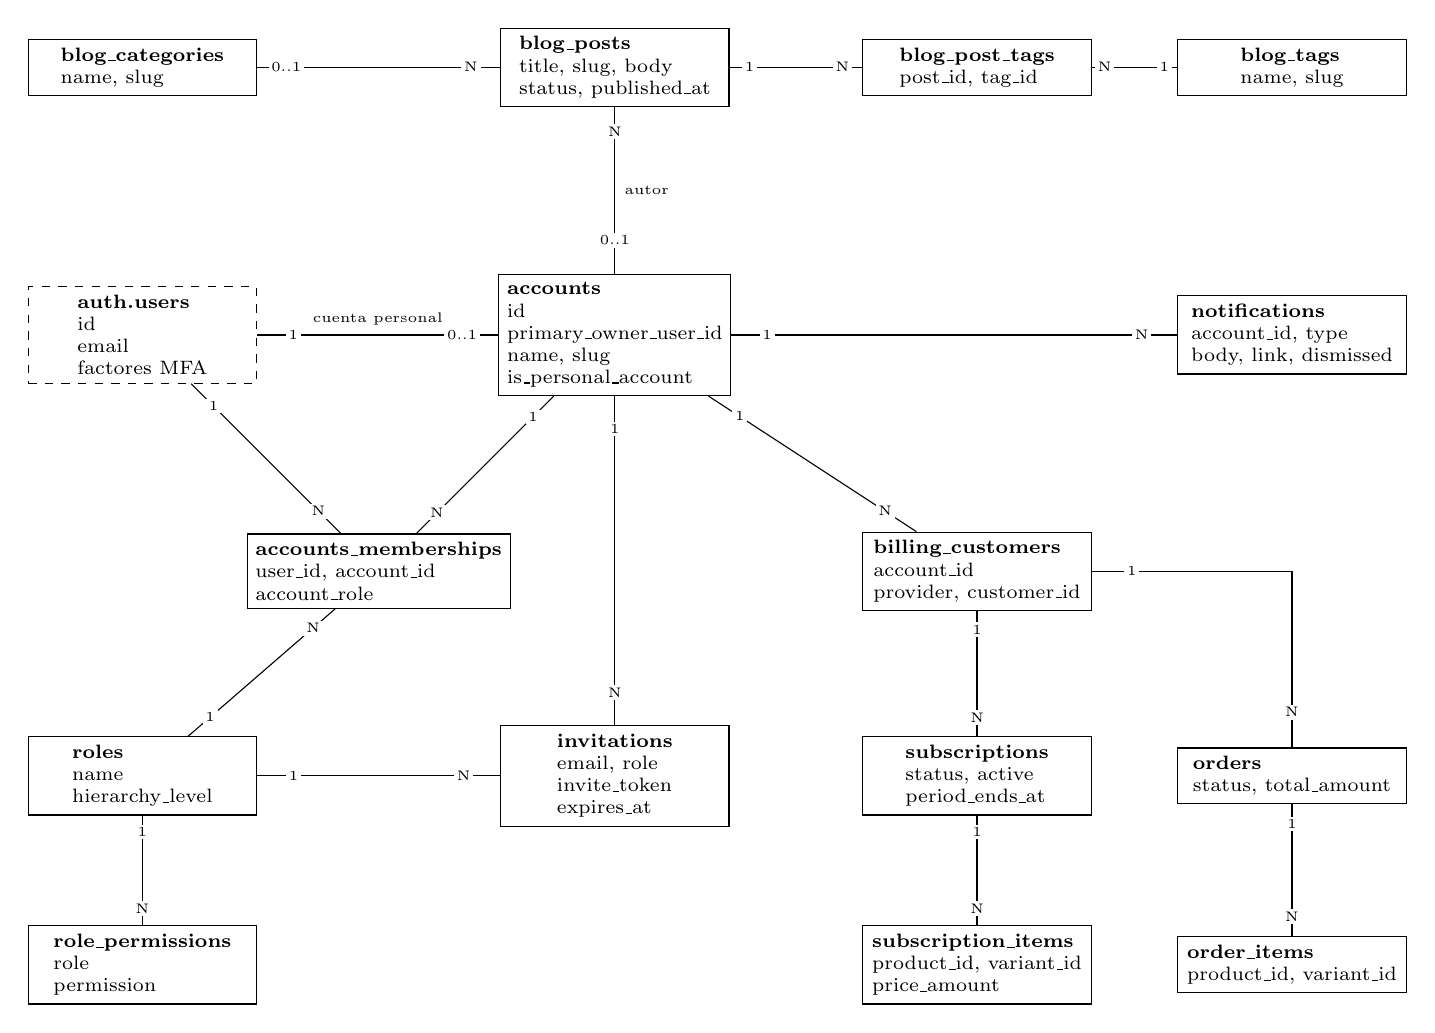
\begin{tikzpicture}[
      font=\scriptsize,
      ent/.style={draw, rectangle, align=left, inner sep=3pt,
                  minimum width=2.9cm, fill=white},
      ext/.style={ent, dashed},
      rel/.style={-},
      card/.style={font=\tiny, inner sep=1pt, fill=white}
    ]
    % Identidad y cuentas
    \node[ext] (users) at (-6, 0) {\textbf{auth.users}\\id\\email\\factores MFA};
    \node[ent] (acc) at (0, 0) {\textbf{accounts}\\id\\primary\_owner\_user\_id\\name, slug\\is\_personal\_account};
    \node[ent] (mem) at (-3, -3) {\textbf{accounts\_memberships}\\user\_id, account\_id\\account\_role};
    \node[ent] (roles) at (-6, -5.6) {\textbf{roles}\\name\\hierarchy\_level};
    \node[ent] (rp) at (-6, -8) {\textbf{role\_permissions}\\role\\permission};
    \node[ent] (inv) at (0, -5.6) {\textbf{invitations}\\email, role\\invite\_token\\expires\_at};

    % Facturación
    \node[ent] (bc) at (4.6, -3) {\textbf{billing\_customers}\\account\_id\\provider, customer\_id};
    \node[ent] (sub) at (4.6, -5.6) {\textbf{subscriptions}\\status, active\\period\_ends\_at};
    \node[ent] (si) at (4.6, -8) {\textbf{subscription\_items}\\product\_id, variant\_id\\price\_amount};
    \node[ent] (ord) at (8.6, -5.6) {\textbf{orders}\\status, total\_amount};
    \node[ent] (oi) at (8.6, -8) {\textbf{order\_items}\\product\_id, variant\_id};

    % Notificaciones
    \node[ent] (not) at (8.6, 0) {\textbf{notifications}\\account\_id, type\\body, link, dismissed};

    % Blog
    \node[ent] (bp) at (0, 3.4) {\textbf{blog\_posts}\\title, slug, body\\status, published\_at};
    \node[ent] (bcat) at (-6, 3.4) {\textbf{blog\_categories}\\name, slug};
    \node[ent] (bpt) at (4.6, 3.4) {\textbf{blog\_post\_tags}\\post\_id, tag\_id};
    \node[ent] (btag) at (8.6, 3.4) {\textbf{blog\_tags}\\name, slug};

    % Relaciones
    \draw[rel] (users) -- node[card, pos=0.15]{1} node[card, pos=0.85]{0..1} node[above, font=\tiny, pos=0.5]{cuenta personal} (acc);
    \draw[rel] (users) -- node[card, pos=0.15]{1} node[card, pos=0.85]{N} (mem);
    \draw[rel] (acc) -- node[card, pos=0.15]{1} node[card, pos=0.85]{N} (mem);
    \draw[rel] (mem) -- node[card, pos=0.15]{N} node[card, pos=0.85]{1} (roles);
    \draw[rel] (roles) -- node[card, pos=0.15]{1} node[card, pos=0.85]{N} (rp);
    \draw[rel] (acc) -- node[card, pos=0.1]{1} node[card, pos=0.9]{N} (inv);
    \draw[rel] (inv.west) -- node[card, pos=0.15]{N} node[card, pos=0.85]{1} (roles.east |- inv.west);
    \draw[rel] (acc) -- node[card, pos=0.15]{1} node[card, pos=0.85]{N} (bc);
    \draw[rel] (bc) -- node[card, pos=0.15]{1} node[card, pos=0.85]{N} (sub);
    \draw[rel] (sub) -- node[card, pos=0.15]{1} node[card, pos=0.85]{N} (si);
    \draw[rel] (bc.east) -| node[card, pos=0.1]{1} node[card, pos=0.9]{N} (ord.north);
    \draw[rel] (ord) -- node[card, pos=0.15]{1} node[card, pos=0.85]{N} (oi);
    \draw[rel] (acc) -- node[card, pos=0.08]{1} node[card, pos=0.92]{N} (not);
    \draw[rel] (bp) -- node[card, pos=0.15]{N} node[card, pos=0.8]{0..1} node[right, font=\tiny, pos=0.5]{autor} (acc);
    \draw[rel] (bp) -- node[card, pos=0.12]{N} node[card, pos=0.88]{0..1} (bcat);
    \draw[rel] (bp) -- node[card, pos=0.15]{1} node[card, pos=0.85]{N} (bpt);
    \draw[rel] (bpt) -- node[card, pos=0.15]{N} node[card, pos=0.85]{1} (btag);
  \end{tikzpicture}}
  \caption{Modelo conceptual de las entidades de la plataforma (esquema
    \texttt{public}). La entidad de trazo discontinuo pertenece al servicio
    de autenticación.}
  \label{fig:ana-datos-public}
  % Texto alternativo: la cuenta (accounts) es el centro del modelo. Cada
  % usuario de auth.users tiene a lo sumo una cuenta personal con su mismo
  % identificador y puede pertenecer a varias cuentas mediante
  % accounts_memberships, que asigna un rol (roles) con sus permisos
  % (role_permissions). Las cuentas tienen invitaciones (con un rol),
  % notificaciones y clientes de facturación, de los que cuelgan
  % suscripciones con sus líneas y pedidos con sus líneas. Las entradas del
  % blog tienen una categoría opcional, un autor (cuenta) opcional y varias
  % etiquetas a través de blog_post_tags.
\end{figure}

La \textbf{cuenta} (\texttt{accounts}) es la unidad de aislamiento
(\textit{tenant}): toda entidad de negocio se enlaza a ella mediante una
columna \texttt{account\_id}. Una cuenta es personal (una por usuario, con su
mismo identificador) o de equipo (con un propietario principal y varios
miembros). Los roles forman una jerarquía mediante
\texttt{hierarchy\_level} y cada uno tiene un conjunto de permisos por
funcionalidad (\texttt{roles.manage}, \texttt{billing.manage},
\texttt{settings.manage}, \texttt{members.manage} e \texttt{invites.manage}).
Por defecto hay tres roles: propietario (\textit{owner}), con todos los
permisos; encargado (\textit{manager}), que gestiona al personal y las
invitaciones pero no la facturación; y miembro (\textit{member}) (ADR-024).
El contenido del blog es la única información pensada para lectura
anónima.

\begin{figure}[htbp]
  \centering
  \resizebox{\textwidth}{!}{%
  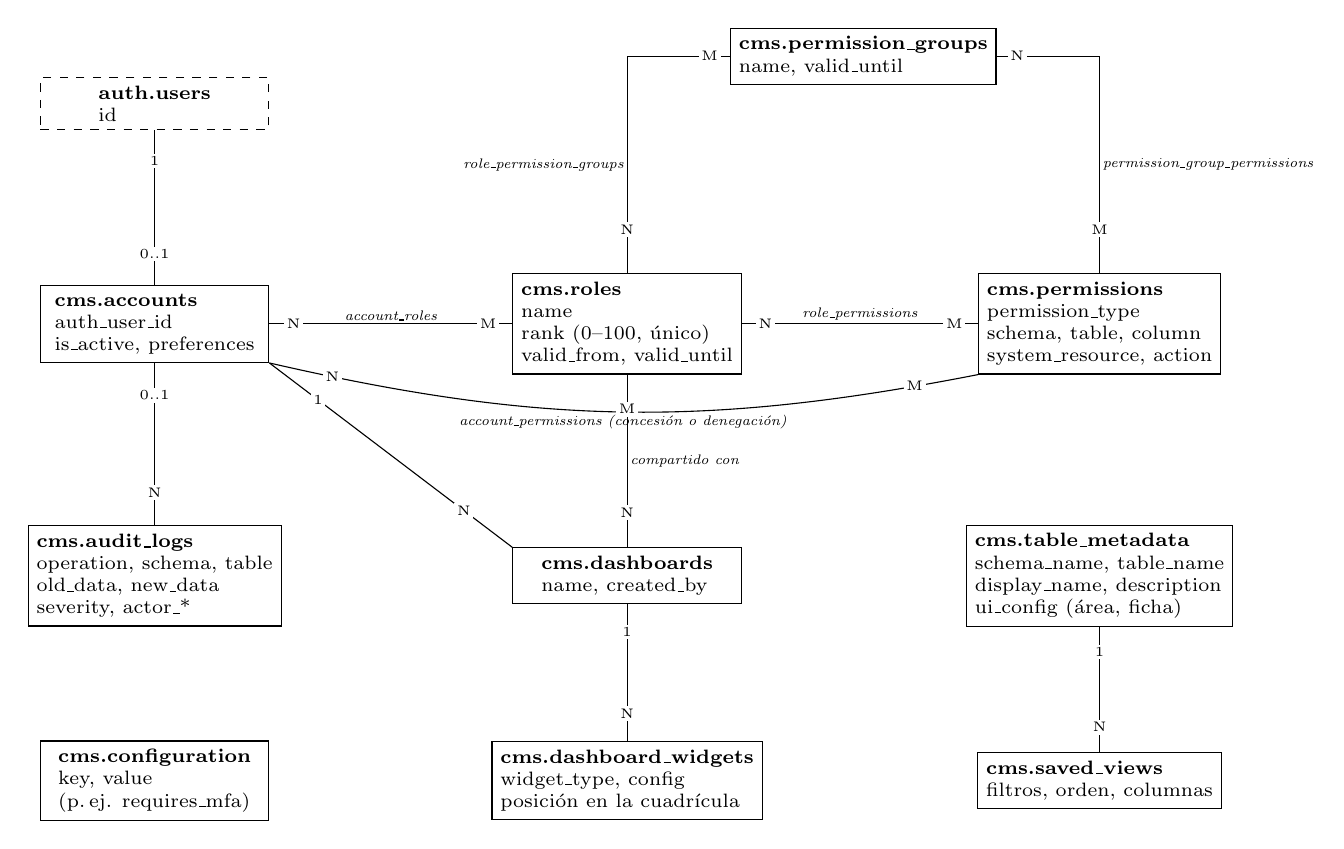
\begin{tikzpicture}[
      font=\scriptsize,
      ent/.style={draw, rectangle, align=left, inner sep=3pt,
                  minimum width=2.9cm, fill=white},
      ext/.style={ent, dashed},
      rel/.style={-},
      card/.style={font=\tiny, inner sep=1pt, fill=white},
      lab/.style={font=\tiny\itshape, fill=white, inner sep=1pt}
    ]
    \node[ext] (users) at (-6, 2.8) {\textbf{auth.users}\\id};
    \node[ent] (cacc) at (-6, 0) {\textbf{cms.accounts}\\auth\_user\_id\\is\_active, preferences};
    \node[ent] (croles) at (0, 0) {\textbf{cms.roles}\\name\\rank (0--100, único)\\valid\_from, valid\_until};
    \node[ent] (cperm) at (6, 0) {\textbf{cms.permissions}\\permission\_type\\schema, table, column\\system\_resource, action};
    \node[ent] (cgroups) at (3, 3.4) {\textbf{cms.permission\_groups}\\name, valid\_until};
    \node[ent] (audit) at (-6, -3.2) {\textbf{cms.audit\_logs}\\operation, schema, table\\old\_data, new\_data\\severity, actor\_*};
    \node[ent] (dash) at (0, -3.2) {\textbf{cms.dashboards}\\name, created\_by};
    \node[ent] (widg) at (0, -5.8) {\textbf{cms.dashboard\_widgets}\\widget\_type, config\\posición en la cuadrícula};
    \node[ent] (meta) at (6, -3.2) {\textbf{cms.table\_metadata}\\schema\_name, table\_name\\display\_name, description\\ui\_config (área, ficha)};
    \node[ent] (views) at (6, -5.8) {\textbf{cms.saved\_views}\\filtros, orden, columnas};
    \node[ent] (conf) at (-6, -5.8) {\textbf{cms.configuration}\\key, value\\(p.\,ej. requires\_mfa)};

    \draw[rel] (users) -- node[card, pos=0.2]{1} node[card, pos=0.8]{0..1} (cacc);
    \draw[rel] (cacc) -- node[card, pos=0.1]{N} node[card, pos=0.9]{M} node[lab, above, pos=0.5]{account\_roles} (croles);
    \draw[rel] (croles) -- node[card, pos=0.1]{N} node[card, pos=0.9]{M} node[lab, above, pos=0.5]{role\_permissions} (cperm);
    \draw[rel] (croles.north) |- node[card, pos=0.1]{N} node[card, pos=0.9]{M} node[lab, pos=0.25, left]{role\_permission\_groups} (cgroups.west);
    \draw[rel] (cgroups.east) -| node[card, pos=0.1]{N} node[card, pos=0.9]{M} node[lab, pos=0.75, right]{permission\_group\_permissions} (cperm.north);
    \draw[rel] (cacc.south east) to[bend right=12] node[card, pos=0.08]{N} node[card, pos=0.92]{M}
      node[lab, below, pos=0.5]{account\_permissions (concesión o denegación)} (cperm.south west);
    \draw[rel] (audit) -- node[card, pos=0.2]{N} node[card, pos=0.8]{0..1} (cacc);
    \draw[rel] (dash.north west) -- node[card, pos=0.2]{N} node[card, pos=0.8]{1} (cacc.south east);
    \draw[rel] (dash) -- node[card, pos=0.2]{1} node[card, pos=0.8]{N} (widg);
    \draw[rel] (dash.north) -- node[card, pos=0.2]{N} node[card, pos=0.8]{M} node[lab, right, pos=0.5]{compartido con} (croles.south);
    \draw[rel] (meta) -- node[card, pos=0.2]{1} node[card, pos=0.8]{N} (views);
  \end{tikzpicture}}
  \caption{Modelo conceptual del esquema \texttt{cms}: control de acceso del
    personal, auditoría, paneles y metadatos de las tablas administradas.}
  \label{fig:ana-datos-cms}
  % Texto alternativo: cada usuario puede tener una cuenta del CMS. Las
  % cuentas tienen roles (con rango único) y los roles tienen permisos,
  % directamente o mediante grupos de permisos; además, una cuenta puede
  % recibir concesiones o denegaciones individuales. La auditoría, los
  % paneles (con sus widgets y compartidos con roles) y las vistas guardadas
  % se relacionan con las cuentas y con los metadatos de tabla, que guardan
  % el nombre visible, la descripción, el área de navegación y el diseño de
  % la ficha de cada tabla. La configuración guarda opciones globales, como
  % la obligatoriedad del MFA.
\end{figure}

El esquema \texttt{cms} añade un segundo modelo de autorización, pensado para
el personal y no para los clientes. Sus permisos son de tres clases:
\emph{de datos} (acción sobre un esquema, una tabla o una columna, con
comodines), \emph{de sistema} (por ejemplo, gestionar miembros o
configuración) y \emph{de almacenamiento} (por contenedor y prefijo de
ruta). Los roles tienen un rango único entre 0 y 100, y todos los permisos,
roles y grupos pueden tener un periodo de vigencia. Los metadatos de tabla
(\texttt{cms.table\_metadata}) son el mecanismo de reutilización del CMS: el
nombre visible, la descripción, el área de la barra lateral y el diseño de
la ficha de cada tabla son \emph{datos}, no código, y se cambian desde la
propia consola (ADR-020).

% ---------------------------------------------------------------------
\section{Reglas de negocio}
\label{sec:ana-reglas}

La tabla~\ref{tab:ana-reglas} recoge las reglas de negocio que el sistema
aplica. Todas se hacen cumplir en la base de datos (restricciones,
\textit{triggers}, políticas o funciones), además de en la interfaz cuando
procede, y cada una está cubierta por pruebas pgTAP.

\begin{longtable}{@{}l>{\raggedright\arraybackslash}p{10.2cm}l@{}}
  \caption{Reglas de negocio.}\label{tab:ana-reglas}\\
  \toprule
  \textbf{ID} & \textbf{Regla} & \textbf{Req.} \\
  \midrule
  \endfirsthead
  \toprule
  \textbf{ID} & \textbf{Regla} & \textbf{Req.} \\
  \midrule
  \endhead
  \bottomrule
  \endfoot
  RN-01 & Cada usuario tiene exactamente una cuenta personal, con su mismo identificador. & RF-05 \\
  RN-02 & Una cuenta de equipo tiene un único propietario principal, que solo cambia mediante una transferencia explícita de la propiedad. & RF-06 \\
  RN-03 & El \textit{slug} de una cuenta de equipo y el de una entrada del blog son únicos. & RF-06, RF-09 \\
  RN-04 & Un miembro no puede invitar, asignar ni modificar un rol de nivel superior al suyo. & RF-06 \\
  RN-05 & Las escrituras destructivas (borrar invitaciones, expulsar miembros, gestionar la facturación) exigen el permiso correspondiente, no la mera pertenencia a la cuenta. & RF-06, RNF-02 \\
  RN-06 & Una invitación caduca a los siete días; cada cuenta puede crear como máximo 20 invitaciones por hora y tener 50 pendientes. & RF-06 \\
  RN-07 & Los datos de suscripciones y pedidos solo los escribe la sincronización con la pasarela de pago; ningún usuario los modifica con su sesión. & RF-07 \\
  RN-08 & La consola de administración y el CMS exigen sesión con segundo factor (\texttt{aal2}). & RF-08, RF-09 \\
  RN-09 & Un super-administrador es automáticamente la raíz del CMS (rol de rango máximo); solo existe un rol raíz y retirar la condición de super-administrador retira el acceso, conservando la cuenta para la auditoría. & RF-08, RF-09 \\
  RN-10 & En el CMS nadie actúa sobre su propia cuenta ni sobre cuentas de rango igual o superior, y las cuentas raíz no se desactivan ni pierden su rol desde la consola. & RF-09 \\
  RN-11 & Una denegación explícita prevalece sobre cualquier concesión, y solo se puede delegar un permiso que se tiene y que no se solapa con ninguna denegación propia. & RF-09, RNF-02 \\
  RN-12 & El MFA del CMS es obligatorio por defecto; solo una cuenta raíz con sesión \texttt{aal2} puede desactivarlo, y el cambio queda auditado. & RF-09, RF-10 \\
  RN-13 & La auditoría solo la escriben las funciones del sistema, con el autor tomado de la sesión; una escritura cuya auditoría falla se deshace. & RF-10 \\
  RN-14 & La auditoría conserva una instantánea del autor aunque se borre su cuenta (ADR-018). & RF-10 \\
  RN-15 & Un \textit{widget} de un panel solo muestra datos de tablas que puede leer quien lo ve, aunque el panel esté compartido. & RF-11 \\
  RN-16 & En la web pública solo es visible una entrada del blog publicada cuya fecha de publicación ya se ha alcanzado. & RF-01 \\
  RN-17 & Los esquemas del sistema (\texttt{auth}, catálogos de PostgreSQL y otros protegidos) nunca se exploran ni se buscan desde el CMS. & RF-09, RNF-02 \\
\end{longtable}
